\chapter{Problem analysis}
\chlab{problems}

Biomolecular simulations are becoming increasingly important for drug development. In these simulations, force field models are required to describe the interatomic relations of the drug molecules. In order to run a simulation, these force fields require a certain topology, which should include the atom types, bonds, angles, atomic charges and charge group assignments.

%Often used force field models include \verb|AMBER|, \verb|CHARMM|, \verb|GROMACS|, \verb|GROMOS| and \verb|OPLS|. 

\begin{figure}[h!]
\begin{center}
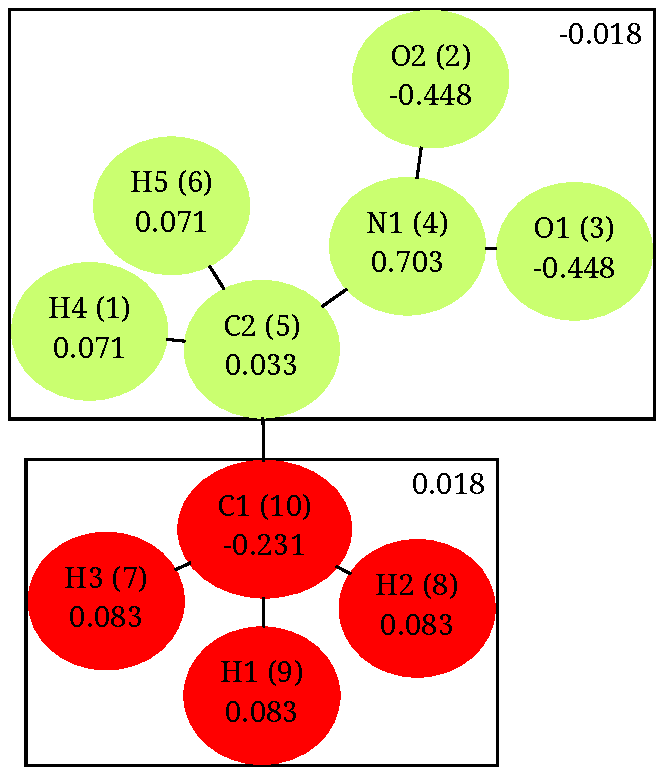
\includegraphics[width=.4\textwidth]{img/partial_charges.pdf}
\caption{Schematic view of nitroethane ($C_{2}H_{5}NO_{2}$), including all topology data.}
\figlab{partial_charges}
\end{center}
\end{figure}

\Figref{partial_charges} shows the schematic view of a nitroethane molecule. Here, every oval symbolises an atom. The atom type is the letter on the top rule of the oval, i.e. \verb|H| is the atom type of the sphere \verb|H5 (6)|. The first number indicates the index in the list of atoms of that type (\verb|5| in the example), the second the overall atom index in the molecule (\verb|6| in the example). The bonds between atoms are shown as lines between the ovals and the atomic charges are given by the number at the bottom row of the oval (\verb|0.071| for \verb|H5 (6)|). Finally, the colouring of the atoms and the squares around them denote a molecular charge group. This is a group of connected atoms, for which the total charge is ideally equal to that of the whole molecule.

In a recent study, El-Kebir, Klau et al. have developed an algorithm that allows for fast and reasonable assignment of charge groups~\cite{canzar2012charge}. As this is now optimised, they currently focus on a different step in the parameterisation: that of calculating the atomic partial charges. Currently, these charges are retrieved using some complex quantum-mechanical calculations. However, as molecules grow bigger, these calculations can take hours or even days to complete. As it is not believed that these calculations can be speeded up, a different approach is needed for finding the partial atomic charges.
% 'Speeded up' is the correct past tense of 'speed up', rather than 'sped up'

One possible way of doing this is by exploiting the similarity of molecules. As similar sections in molecules often have roughly the same atomic charges, it is possible to retrieve the partial charges of an unparameterised molecule from similar sections in other molecules for which the charges \emph{are} known. An algorithm for finding these similar sections is currently being developed at the CWI. However, finding the \emph{best} matches is something only experienced chemists can do. A tool is needed that provides them with a view of the unparameterised molecule and the found related sections. They should then be able to select the best matching sections, and manually adjust some values if this is really needed.

Challenges arise here for the interaction design of the tool. It should be possible to easily compare the related sections, both with each other and with the unparameterised molecule. It should be encouraged to compare more related sections in order to find the best match. This should therefore not take up too much time. As the molecules that will be analysed can vary in size from a few atoms to a few hundred, visualisations should be given some thought to make sure both large and small molecules look good. Overall, the tool should work intuitively and make chemists' work easier, not harder.
